\begin{figure}[h]
    \centering
        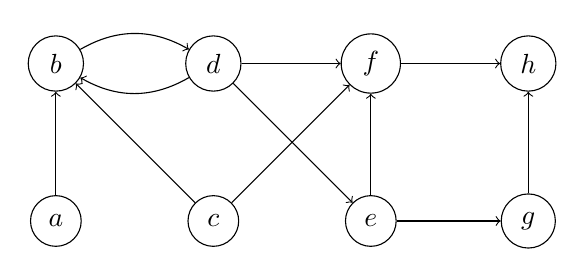
\begin{tikzpicture}
            \tikzset{
                vertex/.style={draw, circle, text width=8, align=center},
                arc/.style={->}
            }

            \draw node[vertex] (a) at (0,0) {$a$};
            \draw node[vertex] (b) at (0,2) {$b$};
            \draw node[vertex] (c) at (2,0) {$c$};
            \draw node[vertex] (d) at (2,2) {$d$};
            \draw node[vertex] (e) at (4,0) {$e$};
            \draw node[vertex] (f) at (4,2) {$f$};
            \draw node[vertex] (g) at (6,0) {$g$};
            \draw node[vertex] (h) at (6,2) {$h$};

            \foreach \x/\y in {%
                a/b,d/f,e/f,c/b,g/h,f/h,d/e,e/g,c/f%
            }{
                \draw (\x) edge[arc] (\y);
            }

            \draw (b) edge[arc, bend left] (d);
            \draw (d) edge[arc, bend left] (b);
        \end{tikzpicture}
        \caption{\label{fig:graph} Graph for Problem 1.}
\end{figure}

\begin{prob}
    Consider a \emph{breadth}-first search on the graph shown in
    Figure~\ref{fig:graph}, starting with node $c$.
    For each node in the graph, write down the distance and predecessor found by the
    BFS.

    \begin{soln}
        % write your solution here
    \end{soln}
\end{prob}
